\documentclass[12pt]{article}
%\usepackage[utf8]{inputenc}
%\documentclass[UTF8]{ctexart}
%\usepackage[UTF8, heading = false, scheme = plain]{ctex}
\usepackage{geometry}
%geometry{a4paper,scale=0.9}
\geometry{a4paper,left=1cm,right=1cm,top=1cm,bottom=2cm}
\usepackage{amsfonts}
\usepackage{color}
\usepackage{url}
%\usepackage{biblatex}
\usepackage{amsmath}
\usepackage{amssymb}
\usepackage{latexsym}
\usepackage{cite}
%\addbibresource{ref.bib}
%\bibliography{ref.bib}
\usepackage{caption}
\usepackage{graphicx, subfig}
\usepackage{float}
%\usepackage[fontset=ubuntu]{ctex}
%\usepackage{fontspec}
\usepackage{xeCJK}
%\usepackage[colorlinks,
%anchorcolor=black,
%citecolor=black]{hyperref}
%\setmainfont{SimSun}
\usepackage[section]{placeins}
\usepackage{enumitem}
\usepackage{framed}
\usepackage[framemethod=TikZ]{mdframed}
\usepackage{indentfirst}
\usepackage{setspace}%使用间距宏包
\linespread{1.5}
%\title{预备知识}
%\author{leolinuxer }
%\date{June 2020}

\title{常见公式}
\author{leolinuxer}
%\date{June 2020}

\begin{document}
\maketitle

\section{初等数学}
\subsection{排列组合}
$$
A_n^m = n(n-1)(n-1) \cdots (n-m+1) = \frac{n!}{(n-m)!}
$$
$$
C_n^m = \frac{A_n^m}{m!} = \frac{n!}{m!(n-m)!}
$$
$$
C_n^m = C_n^{(n-m)}
$$

二项式定理:
$$
(a+b)^n = \sum_{i=0}^n{C_n^ia^{n-i}b^i}
$$

\section{三角函数}
和差角
$$
\sin(\alpha + \beta) = \sin(\alpha)\cos(\beta) + \cos(\alpha)\sin(\beta)
$$
$$
\sin(\alpha - \beta) = \sin(\alpha)\cos(\beta) - \cos(\alpha)\sin(\beta)
$$
$$
\cos(\alpha + \beta) = \cos(\alpha)\cos(\beta) - \sin(\alpha)\sin(\beta)
$$
$$
\cos(\alpha - \beta) = \cos(\alpha)\cos(\beta) + \sin(\alpha)\sin(\beta)
$$
$$
\tan(\alpha + \beta) = \frac{\tan(\alpha) + \tan(\beta))}{1 - \tan(\alpha)\tan(\beta)}
$$
$$
\tan(\alpha - \beta) = \frac{\tan(\alpha) - \tan(\beta))}{1 + \tan(\alpha)\tan(\beta)}
$$

和差化积
$$
\sin(\alpha) + \sin(\beta) = 2\sin(\frac{\alpha + \beta}{2})\cos(\frac{\alpha - \beta}{2})
$$
$$
\sin(\alpha) - \sin(\beta) = 2\sin(\frac{\alpha - \beta}{2})\cos(\frac{\alpha + \beta}{2})
$$
$$
\cos(\alpha) + \cos(\beta) = 2\cos(\frac{\alpha + \beta}{2})\cos(\frac{\alpha - \beta}{2})
$$
$$
\cos(\alpha) - \cos(\beta) = -2\sin(\frac{\alpha + \beta}{2})\sin(\frac{\alpha - \beta}{2})
$$
$$
\tan(\alpha) + \tan(\beta) = \frac{\sin(\alpha + \beta)}{\cos(\alpha)\cos(\beta)}
$$
$$
\tan(\alpha) - \tan(\beta) = \frac{\sin(\alpha - \beta)}{\cos(\alpha)\cos(\beta)}
$$

积化和差
$$
\sin(\alpha)\cos(\beta) = \frac{\sin(\alpha + \beta) + \sin(\alpha - \beta)}{2} 
$$
$$
\cos(\alpha)\sin(\beta) = \frac{\sin(\alpha + \beta) - \sin(\alpha - \beta)}{2} 
$$
$$
\cos(\alpha)\cos(\beta) = \frac{\cos(\alpha + \beta) + \cos(\alpha - \beta)}{2} 
$$
$$
\sin(\alpha)\sin(\beta) = -\frac{\cos(\alpha + \beta) - \cos(\alpha - \beta)}{2} 
$$

二倍角公式
$$
\sin(2\alpha) = 2\sin(\alpha)\cos(\alpha)
$$
$$
\cos(2\alpha) = 2\cos^2(\alpha) - 1 = 1 - 2\sin^2(\alpha) = \cos^2(\alpha) - \sin^2(\alpha)
$$
$$
\tan(2\alpha) = \frac{2\tan(\alpha)}{1 - \tan^2(\alpha)}
$$

万能公式
设
$$
\tan(\frac{\alpha}{2}) = t, \quad \alpha \neq 2k\pi + \pi, k \in Z
$$
$$
\sin(\alpha) 
= \frac{2\sin(\alpha/2)\cos(\alpha/2)}{\sin^2(\alpha/2) + \cos^2(\alpha/2)} 
= \frac{2t}{1+t^2} 
$$
$$
\cos(\alpha) 
= \frac{\cos^2(\alpha/2) - \sin^2(\alpha/2)}{\sin^2(\alpha/2) + \cos^2(\alpha/2)} 
= \frac{1-t^2}{1+t^2} 
$$
$$
\tan(\alpha) = \frac{2\tan(\alpha/2)}{1 - \tan^2(\alpha/2)} = \frac{2t}{1-t^2}
$$

就是说$\sin(\alpha),\cos(\alpha),\tan(\alpha)$都可以用$\tan(\alpha/2)$来表示,当要求一串函数式最值的时候,就可以用万能公式,推导成只含有一个变量的函数,最值就很好求了.

\begin{framed}  
%\verb|\documentstyle[ifthen,12pt,titlepage]{article}|
\small{
$f(x) = \sin(2x) + 2\sin(x)$,求最大值
\begin{align*}
|f(x)| &= |2\sin(x)\cos(x) + 2\sin(x)| \\
    &= 2|\sin(x)(\cos(x) + 1)| \\
    &= 2|2\sin(\frac{x}{2})\cos(\frac{x}{2})\cdot 2\cos^2(\frac{x}{2})| \\
    &= \frac{8}{\sqrt{3}}\sqrt{(3\sin^2(\frac{x}{2}))(\cos^2(\frac{x}{2}))(\cos^2(\frac{x}{2}))(\cos^2(\frac{x}{2}))} \\
    &\le \frac{8}{\sqrt{3}}\sqrt{[\frac{(3\sin^2(\frac{x}{2})) + (\cos^2(\frac{x}{2})) + (\cos^2(\frac{x}{2})) + (\cos^2(\frac{x}{2}))}{4}]^4} \\
    &= \frac{8}{\sqrt{3}}\cdot \frac{9}{16} \\
    &= \frac{3\sqrt{3}}{2} 
\end{align*}

另,采用万能公式计算:
$$
f(x) = \sin(2x) + 2\sin(x)
$$
$$
f(t) = 2\cdot\frac{2t}{1+t^2}\cdot\frac{1-t^2}{1+t^2} + 2\cdot\frac{2t}{1+t^2} = \cdots = \frac{8t}{(1+t^2)^2}
$$
$$
f'(t) = \frac{8t}{(1+t^2)^2} - \frac{32t^2}{(1+t^2)^3} = \frac{8-32t^2}{(1+t^2)^3}
$$

令$f'(t) = 0$,有 $t = \frac{\sqrt{3}}{3}$

所以 $f(t)_{max} = f(\frac{\sqrt{3}}{3}) = \frac{3\sqrt{3}}{2}$
}
\end{framed}

\section{复数}
复数的\textbf{代数表示式}:
$$
z = a + bi, \quad a,b \in R
$$

复数的\textbf{三角表示式}:
$$
z = r(\cos\theta + i\sin\theta)
$$

复数的\textbf{指数表示式(欧拉公式)}:
$$
z = e^{i\theta} = \cos\theta + i\sin\theta
$$

令$\theta=\pi$,可以得到\textbf{欧拉魔幻等式}:
$$
e^{i\pi} + 1 = 0
$$

利用指数表示式,有:
$$
e^{i\theta_1} \cdot e^{i\theta_2} = (\cos\theta_1 + i\sin\theta_1)\cdot(\cos\theta_2 + i\sin\theta_2) = e^{i(\theta_1+\theta_2)}
$$

同时,有:
$$
(e^{i\theta})^n = e^{in\theta}
$$

圆上的欧拉公式如下图:
\begin{figure}[H]
  \centering
  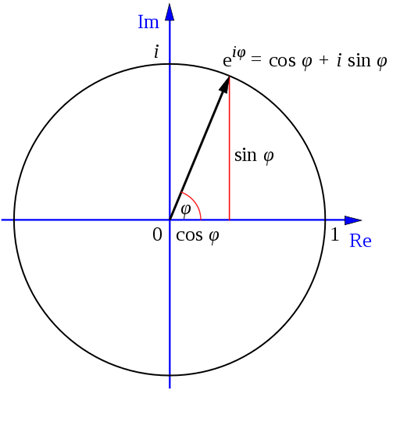
\includegraphics[width=.3\textwidth]{fig/EulerEquationInCircle.png} 
\end{figure}

\section{极限和微积分相关}
\subsection{一些级数的和}
$$
\sum_{k=1}^{n}k^2 = 1^2 + 2^2 + \cdots + n^2 = \frac{n(n+1)(2n+1)}{6}
$$

\subsection{圆周率$\pi$ 的相关公式}
圆周率$\pi$ 的公式:
$$
    \frac{\pi}{4} = 1 - \frac{1}{3} + \frac{1}{5} - \frac{1}{7} \cdots
$$

$$
    \frac{\pi^2}{6} = 1 + \frac{1}{2^2} + \frac{1}{3^2} + \frac{1}{4^2} \cdots
$$

$$
\frac{\pi}{4} = \int_0^1\frac{1}{x^2+1}dx
$$

\subsection{关于$e$}
$$
e = (1 + \frac{1}{n})^n \quad n \to \infty
$$

\subsection{积分运算的规则}
$$
\int_a^b[cf(x) + dg(x)]dx = c\int_a^bf(x)dx + d\int_a^bg(x)dx
$$

$$
\int_a^bf(x)dx = -\int_b^af(x)dx
$$

$$
\int_a^bf(x)dx = \int_a^bf(u)du = \int_a^bf(t)dt
$$

\begin{framed}  
%\verb|\documentstyle[ifthen,12pt,titlepage]{article}|
利用上式参数变换的思想,有:
$$
\int_1^bf(x)dx = \int_0^{b-1}du \quad x = x' + 1    
$$

例:若 $n > 0$,证明 $(1+x)^n$ 从 -1 到 z 的积分等于 $\frac{(1+z)^{n+1}}{n+1}$

证明:令 $x' = 1+x$,那么有:
$$
\int_{-1}^z (1+x)^ndx = \int_0^{z+1}{x'}^ndx' = [\frac{{x'}^{n+1}}{n+1}]_0^{z+1} = \frac{(1+z)^{n+1}}{n+1}
$$
\end{framed}

$$
\int_a^bf(x)dx \le \int_a^b|f(x)|dx
$$

$$
|\int_a^bf(x)dx| \le \int_a^b|f(x)|dx
$$

\subsection{常见导数公式}
\begin{table}[H]
    \centering
    \begin{tabular}{|c|c|}
    \hline 
       原函数    & 导函数  \\ \hline
       链式法则 $y = f[g(x)]$ & $y' = f'[g(x)]\times g'(x)$ \\ \hline
       反函数求导法则:若 $y=f(x) $ 的反函数是 $x = g(y)$ & $y' = \frac{1}{x'}$ \\ \hline
       $y = uv$  & $y' = u'v + uv'$ \\ \hline
       $y = \frac{u}{v}$ & $y' = \frac{u'v - uv'}{v^2}$ \\ \hline
       $y=c$     & $y'=0$ \\ \hline
       $y = n^x$ & $y' = n^x\ln{x} $ \\ \hline
       $y = \log_ax$ & $y' = \frac{1}{\ln{a}}$ \\ \hline
       $y = \ln{x} $ & $y' = \frac{1}{x}$ \\ \hline
       $y = x^n$ & $y' = nx^{n-1}$ \\ \hline
       $y = \sin{x}$ & $y' = \cos{x}$ \\ \hline
       $y = \cos{x}$ & $y' = -\sin{x}$ \\ \hline
       $y = \tan{x}$ & $y' = \frac{1}{\cos{x}^2} = \sec{x}^2$ \\ \hline
       $y = \cot{x}$ & $y' = -\frac{1}{\sin{x}^2} = -\csc{x}^2$ \\ \hline
       $y = \arcsin{x}$ & $y' = \frac{1}{\sqrt{1-x^2}}$ (利用反函数求导法则)\\ \hline
       $y = \arccos{x}$ & $y' = -\frac{1}{\sqrt{1-x^2}}$ \\ \hline
       $y = \arctan{x}$ & $y' = \frac{1}{1+x^2}$ \\ \hline
       $y = arccot{x}$ & $y' = -\frac{1}{1+x^2}$ \\ \hline
       $y = arcsec{x}$ & $y' = \frac{1}{x\sqrt{x^2-1}}$ \\ \hline
       $y = arccsc{x}$ & $y' = -\frac{1}{x\sqrt{x^2-1}}$ \\ \hline
       $y = sh{x} = \frac{e^x - e^{-x}}{x}$ & $y' = ch{x}$ \text{双曲函数} \\ \hline
       $y = ch{x} = \frac{e^x + e^{-x}}{2}$ & $y' = sh{x}$ \\ \hline
       $y = th{x} = \frac{e^x - e^{-x}}{e^x + e^{-x}}$ & $y' = \frac{1}{ch{x}^2}$ \\ \hline
       $y = arsh{x} = \ln{(x + \sqrt{x^2+1})}$ & $y' = \frac{1}{\sqrt{x^2+1}}$ \\ \hline
       $y = arch{x} = \ln{(x+\sqrt{x^2-1})}$ & $y' = \frac{1}{\sqrt{x^2-1}}$ \\ \hline
       $y = arth{x} = \frac{1}{2}\ln(\frac{1+x}{1-x})$ & $y' = \frac{1}{1-x^2}$ \\ \hline
    \end{tabular}
\end{table}

\subsection{泰勒公式}
$$
f(x) = \frac{f(a)}{0!} + \frac{f'(a)}{1!}(x-a) + \frac{f''(x)}{2!}(x-a)^2 + \cdots + \frac{f^{(n)(a)}}{n!}(x-a)^n + R_n(x)
$$

$$
e^x = 1 + x + \frac{x^2}{2!} + \frac{x^3}{3!} + \cdots
$$

$$
\ln(1+x) = x - \frac{x^2}{2} + \frac{x^3}{3} - \cdots + (-1)^{k-1}\frac{x^k}{k} \quad (|x) < 1)
$$

$$
\sin{x} = x - \frac{x^3}{3!} + \frac{x^5}{5!} - \cdots + (-1)^{k-1}\frac{x^{2k-1}}{(2k-1)!}
$$

\subsection{利用积分求无穷级数的和}
对于函数 $f(x)$,它在 $x\in[a,b]$内的面积,用积分可以表示为:
$$
S = \int_a^bf(x)dx
$$
同时,我们将 $x=a$ 到 $x=b$ 的区间分割成 $n$ 个小区间,在每个分点上做垂线,它的高是该垂线的长度,这就构成了 $n$ 个矩形;当 $n \rightarrow \infty $ 时,这些矩形的面积之和就等于 $S$。这些矩形的面积可以组成一个序列:
$$
S_1, S_2, S_3, \cdots
$$
使得当 $n$ 无限增加、$S_n$中最宽的矩形的宽度趋于零时,该序列趋于极限 $A$,
$$
S_n \rightarrow A
$$

这里,$S_n$可以简写成:
$$
S_n = \sum_j^nf(x_j)\Delta x
$$

也就是说,我们可以看出极限和积分的关系为:
$$
A = \lim_{n \rightarrow \infty}\sum_{j=1}^{n}f(x_j)\Delta x = \int_a^bf(x)dx
$$

根据这个思想,我们可以求解一些无穷级数的和。

\begin{framed}  
%\verb|\documentstyle[ifthen,12pt,titlepage]{article}|
\small{
例题:证明当 $n->\infty$ 时,
$$
S = \frac{1^k + 2^k + \cdots + n^k}{n^{k+1}} \rightarrow \frac{1}{k+1}
$$

证明:考虑如下积分:
$$
S = \int_0^1x^kdx
$$

将其在 $[0,1]$ 的区间内,平均分成 $n$ 份,则每份的宽度为 $\Delta x = \frac{1-0}{n} = \frac{1}{n}$,且每份的高度分别为:
\begin{itemize}
    \item $x_1 = \Delta x, y_1 = (\Delta x)^k = (\frac{1}{n})^k$
    \item $x_2 = 2\Delta x, y_2 = (2\Delta x)^k = (\frac{2}{n})^k$
    \item $\cdots$
    \item $x_n = n\Delta x, y_n = (n\Delta x)^k = (\frac{n}{n})^k$
\end{itemize}

所以,面积的和为:
\begin{align}
   S_n &= \Delta x((\Delta x)^k + (2\Delta x)^k + \cdots + (n\Delta x)^k) \\
   &= \frac{1}{n}((\frac{1}{n})^k + (\frac{2}{n})^k + \cdots + (\frac{n}{n})^k) \\
   &= \int_0^1x^kdx = [\frac{x^(k+1)}{k+1}]_0^1 = \frac{1}{k+1}
\end{align}

即:
$$
S = \frac{1^k + 2^k + \cdots + n^k}{n^{k+1}} \rightarrow \frac{1}{k+1} = \int_0^1x^kdx = \frac{1}{k+1}
$$
}
\end{framed}

\begin{framed}  
%\verb|\documentstyle[ifthen,12pt,titlepage]{article}|
\small{
例题:证明当 $n->\infty$ 时,
$$
\frac{1}{\sqrt{n}}(\frac{1}{\sqrt{1+n}} + \frac{1}{\sqrt{2+n}} + \cdots + \frac{1}{\sqrt{n+n}}) \rightarrow 2(\sqrt{2} - 1)
$$

证明:考虑如下积分:
$$
S = \int_0^2\frac{1}{\sqrt{x}}dx \quad \text{(注意,积分区间是} [0,2])
$$

将其在 $[0,2]$ 的区间内,平均分成 $2n$ 份,则每份的宽度为 $\Delta x = \frac{2-0}{2n} = \frac{1}{n}$,且每份的高度分别为:
\begin{itemize}
    \item $x_1 = \Delta x, y_1 = \frac{1}{\sqrt{\Delta x}}$
    \item $x_2 = 2\Delta x, y_1 = \frac{1}{\sqrt{2\Delta x}}$
    \item $x_3 = 3\Delta x, y_1 = \frac{1}{\sqrt{3\Delta x}}$
    \item $\cdots$
    \item $x_n = n\Delta x, y_1 = \frac{1}{\sqrt{n\Delta x}}$
    \item $x_{n+1} = (n+1)\Delta x, y_1 = \frac{1}{\sqrt{(n+1)\Delta x}}$
    \item $\cdots$
    \item $x_{2n} = (2n)\Delta x, y_1 = \frac{1}{\sqrt{(2n)\Delta x}}$
\end{itemize}

所以,面积的和为:
\begin{align}
   S_n &= \Delta x(\frac{1}{\sqrt{\Delta x}} + \frac{1}{\sqrt{2\Delta x}} + \cdots + \frac{1}{\sqrt{n\Delta x}} + \frac{1}{\sqrt{(n+1)\Delta x}} + \cdots + \frac{1}{\sqrt{(2n)\Delta x}}) \\
   &= \sqrt{\Delta x}(\frac{1}{\sqrt{1}} + \frac{1}{\sqrt{2}} + \cdots + \frac{1}{\sqrt{n}} + \frac{1}{\sqrt{n+1}} + \cdots + \frac{1}{\sqrt{2n}}) \\
   &= \frac{1}{\sqrt{n}}(\frac{1}{\sqrt{1}} + \frac{1}{\sqrt{2}} + \cdots + \frac{1}{\sqrt{n}} + \frac{1}{\sqrt{n+1}} + \cdots + \frac{1}{\sqrt{2n}}) \\
   &= \int_0^2\frac{1}{\sqrt{x}}dx = \int_0^2x^{-\frac{1}{2}dx} = [2x^{\frac{1}{2}}]_0^2 = 2\sqrt{2}
\end{align}

也就是说,级数:
$$
\frac{1}{\sqrt{n}}(\frac{1}{\sqrt{1}} + \frac{1}{\sqrt{2}} + \cdots + \frac{1}{\sqrt{n}} + \frac{1}{\sqrt{n+1}} + \cdots + \frac{1}{\sqrt{2n}}) = \int_0^2\frac{1}{\sqrt{x}}dx = 2\sqrt{2}
$$

所以,题目中的级数:
$$
\frac{1}{\sqrt{n}}(\frac{1}{\sqrt{1+n}} + \frac{1}{\sqrt{2+n}} + \cdots + \frac{1}{\sqrt{n+n}}) = \int_0^2\frac{1}{\sqrt{x}}dx - \int_1^2\frac{1}{\sqrt{x}}dx
= 2\sqrt{2} - 2 = 2(\sqrt{2} - 1)
$$
}
\end{framed}

%\printbibliography
\bibliography{../ref}
\bibliographystyle{IEEEtran}
\end{document}
